\documentclass[11pt]{article}
\usepackage[margin=1in]{geometry}
\usepackage{subcaption}
\usepackage{graphicx}
\usepackage{placeins}
\usepackage{amsmath}
\usepackage{url}
\usepackage{cite}
\usepackage{array}
\usepackage{xltabular}
\usepackage{ltablex}
\usepackage{lineno}


% acronyms for text or math mode
% \newcommand {\ccast} {\mbox{\small\textsc{ccast}}}
\newcommand {\ccast} {\mbox{\small CCAST}}
\newcommand {\nedn} {\mbox{\small NEdN}}
\newcommand {\kcarta} {\mbox{k\small{CARTA}}}

\newcommand {\chirp} {\mbox{\small CHIRP}}
\newcommand {\cris}  {\mbox{\small CrIS}}
\newcommand {\airs}  {\mbox{\small AIRS}}
\newcommand {\iasi}  {\mbox{\small IASI}}
\newcommand {\idps}  {\mbox{\small IDPS}}
\newcommand {\nasa}  {\mbox{\small NASA}}
\newcommand {\noaa}  {\mbox{\small NOAA}}
\newcommand {\nstar} {\mbox{\small STAR}}
\newcommand {\umbc}  {\mbox{\small UMBC}}
\newcommand {\uw}    {\mbox{\small UW}}

\newcommand {\fft}  {\mbox{\small FFT}}
\newcommand {\ifft} {\mbox{\small IFFT}}
\newcommand {\fir}  {\mbox{\small FIR}}
\newcommand {\fov}  {\mbox{\small FOV}}
\newcommand {\for}  {\mbox{\small FOR}}
\newcommand {\ict}  {\mbox{\small ICT}}
\newcommand {\ils}  {\mbox{\small ILS}}
\newcommand {\igm}  {\mbox{\small IGM}}
\newcommand {\opd}  {\mbox{\small OPD}}
\newcommand {\rms}  {\mbox{\small RMS}}
\newcommand {\zpd}  {\mbox{\small ZPD}}
\newcommand {\ppm}  {\mbox{\small PPM}}
\newcommand {\srf}  {\mbox{\small SRF}}
\newcommand {\sdr}  {\mbox{\small SDR}}
\newcommand {\FWHM} {\mbox{\small FWHM}}
\newcommand {\fwhm} {\mbox{\small\textsc{fwhm}}}

\newcommand {\ES} {\mbox{\small ES}}
\newcommand {\SP} {\mbox{\small SP}}
\newcommand {\IT} {\mbox{\small IT}}
\newcommand {\SA} {\mbox{\small SA}}

\newcommand {\ET} {\mbox{\small ET}}
\newcommand {\FT} {\mbox{\small FT}}

\newcommand {\wn} {\mbox{cm$^{-1}$}}
\newcommand {\cm} {\mbox{cm}}

% abbreviations, mainly for math mode
\newcommand {\real} {\mbox{real}}
\newcommand {\imag} {\mbox{imag}}
\newcommand {\atan} {\mbox{atan}}
\newcommand {\obs}  {\mbox{obs}}
\newcommand {\calc} {\mbox{calc}}
\newcommand {\sinc} {\mbox{sinc}}
\newcommand {\psinc} {\mbox{psinc}}
\newcommand {\std} {\mbox{std}}
\newcommand {\nchan} {\mbox{nchan}}
\newcommand {\nobs} {\mbox{nobs}}

% symbols, for math mode only
\newcommand {\lmax} {L_{\mbox{\tiny max}}}
\newcommand {\vmax} {V_{\mbox{\tiny max}}}

\newcommand {\tauobs} {\tau_{\mbox{\tiny obs}}}
\newcommand {\taucal} {\tau_{\mbox{\tiny calc}}}
\newcommand {\Vdc}  {V_{\mbox{\tiny DC}}}

\newcommand {\rIT} {r_{\mbox{\tiny\textsc{ict}}}}
\newcommand {\rES} {r_{\mbox{\tiny\textsc{es}}}}
\newcommand {\robs} {r_{\mbox{\tiny obs}}}

\newcommand {\rITobs} {r_{\mbox{\tiny\textsc{ict}}}^{\mbox{\tiny obs}}}
\newcommand {\rITcal} {r_{\mbox{\tiny\textsc{ict}}}^{\mbox{\tiny cal}}}

\newcommand {\rESuser} {r_{\mbox{\tiny\textsc{es}}}^{\mbox{\tiny user}}}
\newcommand {\rITuser} {r_{\mbox{\tiny\textsc{ict}}}^{\mbox{\tiny user}}}
\newcommand {\rITsensor} {r_{\mbox{\tiny\textsc{ict}}}^{\mbox{\tiny sensor}}}
\newcommand {\rITfov} {r_{\mbox{\tiny\textsc{ict}}}^{\mbox{\tiny fov}}}

\newcommand {\fcos} {f_{\mbox{\tiny cos}}}
\newcommand {\fatbd} {f_{\mbox{\tiny\textsc{atbd}}}}

\newcommand {\ITmean} {\langle\mbox{\small IT}\rangle}
\newcommand {\SPmean} {\langle\mbox{\small SP}\rangle}

\newcommand {\Ttc} {t^{\mbox{\tiny\textsc{tc}}}}
\newcommand {\Tac} {t^{\mbox{\tiny\textsc{ac}}}}
\newcommand {\rtc} {r_{\mbox{\tiny\textsc{tc}}}}
\newcommand {\rta} {r_{\mbox{\tiny\textsc{ta}}}}



%\usepackage[T1]{fontenc}
\usepackage[utf8]{inputenc}
\usepackage{beton}% or ccfonts, or concrete

\usepackage[colorlinks=true,
            linkcolor=blue,
            urlcolor=blue,
            citecolor=blue,
            linkbordercolor={0.8 0.8 0.8},
            menubordercolor={0 1 0}]{hyperref}

\newcommand {\radunits} {\hbox{mW sr$^{-1}$ m$^{-2}$}}

\title{
  CHIRP User Guide \\
}
\author{H.~E.~Motteler and L.~L.~Strow \\
  \\
  University of Maryland Baltimore County (UMBC)\\
  Joint Center for Earth Systems Technology \\
  Atmospheric Spectroscopy Lab \\
}
\date{\today}
\begin{document}
\maketitle

\tableofcontents
%\linenumbers

%----------- section --------------------------------------------------%
\section{Introduction}
\label{intro}

Spectra of the earth's thermal emission as measured by the AIRS
\cite{airs1}, CrIS\cite{cris1,cris2}, and IASI \cite{iasi1}
hyper-spectral sounders are a significant part of the long term
climate record.  These instruments have broadly similar spatial
sampling, spectral resolution, and band spans.  But the spectral
response functions differ in detail, leading to significant
differences in observed spectra.
The Climate Hyperspectral Infrared Radiance Product (CHIRP) provides
a single, combined record of these data, by taking advantage of the
similar spatial sampling, translating AIRS and CrIS radiances to a
common spectral response function, and removing inter-satellite
biases.  CHIRP provides a stable climate-quality radiance time
series spanning AIRS, CrIS, and potentially in the future, IASI
radiance data.  Other benefits include facilitating instrument
comparisons and allowing level~2 retrievals to use a common channel
set and radiative transfer algorithm.

The translation from CrIS to CHIRP is done by resampling or double
Fourier interpolation.  Translation from AIRS to CHIRP is more
involved.  AIRS is a grating spectrometer with a distinct response
function for each channel, while CrIS is a Michelson interferometer
with a sinc response function.  We use our knowledge of the AIRS
spectral response functions to deconvolve AIRS channel radiances to
a resolution enhanced intermediate representation, which is then
reconvolved to the CHIRP user grid.  The CrIS instrument on NASA's
SNPP satellite is used as the calibration standard, while a bias
adjustment is applied to the other translations \cite{strow2021a}.

% chirp timeline
\begin{figure}
  \centering
  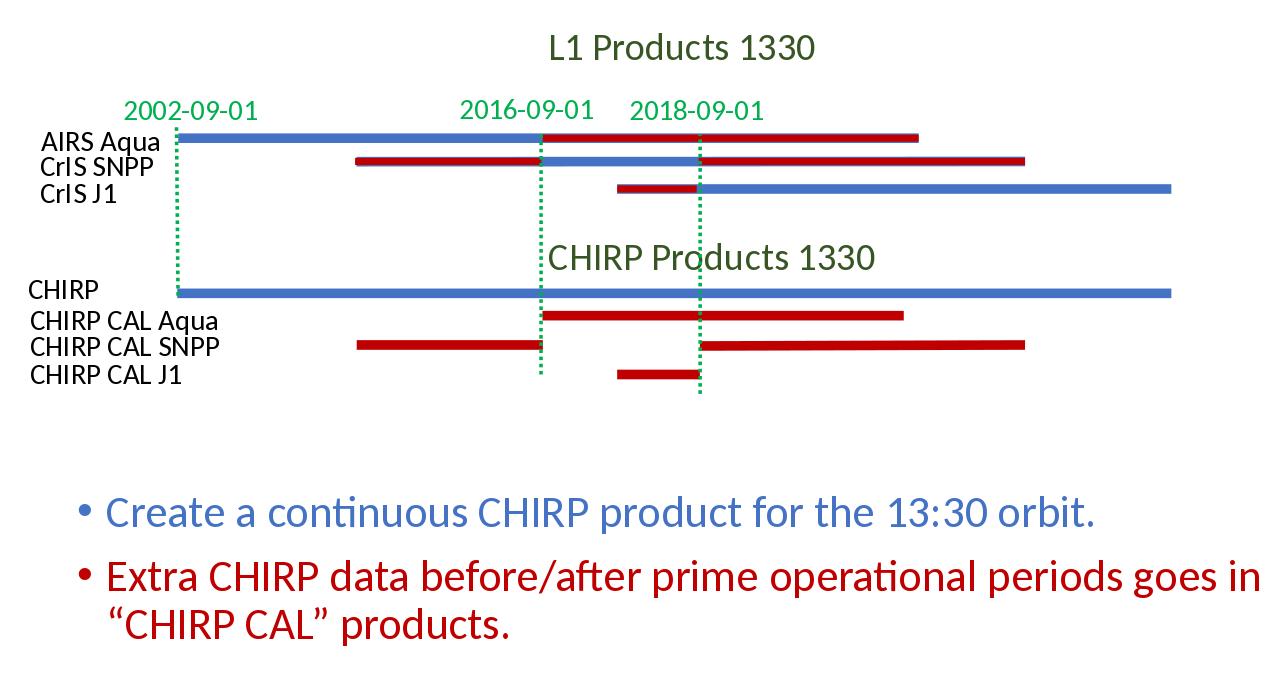
\includegraphics[width=\textwidth]{figures/chirp_timeline.png}
  \caption{Timeline for CHIRP and component products.}
  \label{fig0}
\end{figure}

The CHIRP record starts with AIRS data from Fall 2002, and will cross over
to CrIS SNPP and then CrIS J1 (aka NOAA-20) as shown in figure \ref{fig0}.
This is planned to continue in the future with NOAA-21, 22, etc., with
sounder crossover dates to be determined.  These sounders share an
ascending 1:30 PM (13:30) equatorial crossing time and are combined as
shown in \ref{fig0} to make the CHIRP-1330 product.  Although the primary
product is a single continuous record, support products in the form of
translations for other NOAA sounders and times are also provided as
CHIRP-CAL products.  These support product allow users to create radiance
time series that cross over from one instrument to the next at different
times than the CHIRP-1330 product, as long as the CHIRP-CAL product exists
for the desired times.  For example, a valid time series could use AIRS
parent radiances until AIRS ceases operation, and then switch directly to
CrIS J1 (NOAA-20).

Section \ref{format} is a short introduction to using the CHIRP data.
This is followed by sections with more detail on radiances, sampling,
quality control, and NEdN estimates, and an appendix with tables of
all variables and attributes.  For more detail on the AIRS to CHIRP
translation, see reference \cite{mott2018}, and for more on bias
adjustments and questions of long-term stability, see reference
\cite{strow2021a}.

%----------- section --------------------------------------------------%
\section{Quick Start}
\label{format}

CHIRP data is saved as a sequence of granule files, in time order,
in netCDF format.  A CHIRP observation, or ``obs'' for short, is a
1679-channel radiance vector with associated values for time,
geolocation, latitude, longitude, quality control, and various other
support data.  The key idea is that each such obs can stand alone as
a largely self-sufficient unit of information.  CHIRP data is then
simply a list of such obs, in time order.  The CHIRP radiance data
is organized as a $1679 \times 12150$ array, channels by obs, while
most of the supporting data is organized as $12150$-vectors.  The
choice of 12150 obs per granule is discussed in section
\ref{sampling}.

For example, suppose an application needs radiance, channel
frequency, quality control, obs time, latitude, and longitude.
The CHIRP netCDF fields, data types, and physical units are as
follows:

\begin{itemize}

\item
The CHIRP radiance field is \texttt{rad}, a 1679 by 12150 element
single precision array, in units of \radunits.  Channel frequency is
\texttt{wnum}, a 1679 element double precision vector, in units of
wavenumber.

\item
Quality control fields are \texttt{chan\_qc} and \texttt{rad\_qc}.
\texttt{chan\_qc} is a 1679 element int8 array, one flag per
channel, with 0=OK, 1=Warn, and 2=Bad.  \texttt{rad\_qc} is a 12150
element int8 array, one flag per obs, where again 0=OK, 1=Warn, and
2=Bad.

\item
The time field is \texttt{obs\_time\_tai93}, a 12150 element double
precision vector, seconds since 1 Jan 1993.

\item
The geolocation fields are are \texttt{lat} and \texttt{lon}, 12150
element single precision vectors, with units degrees north and
degrees east.

\end{itemize}

The organization of other support variables is generally similar, and
all CHIRP fields and attributes are defined in appendix \ref{fields}.
The AIRS-parent CHIRP channels are a subset of the CrIS-parent
channels.  The \texttt{wnum} grid is used for both, with missing
AIRS-parent channels flagged as bad.  This is discussed in more
detail in section \ref{qcnedn}.  The parent AIRS and CrIS radiance
data are organized as a sequence of granule files, ordered by scan
geometry and observation time.  See section \ref{sampling} for
details.  CHIRP granules correspond with their parent AIRS or CrIS
granules, and inherit most of the parent granule's attributes and
supporting data.  The stand-alone nature of the CHIRP obs requires
some duplication of information---for example the CrIS-parent data
includes the FOV number for every obs---but the overhead for this is
small in comparison with the space required for the radiance data.

%------------- old text --------------
%
% AIRS L1c and CrIS L1b radiance data are organized as a sequence of
% granule files, ordered by scan geometery and observation time.
% CHIRP granules correspond with their parent AIRS or CrIS granules,
% and inherit most of the parent granule's attributes and supporting
% data.  CHIRP granules follow JPL conventions for field names and
% attributes, and are saved in netCDF.  There are 1679 CHIRP channels,
% described in detail in section \ref{rad}.  A CHIRP observation, or
% ``obs'' for short, is a 1679-channel radiance vector with associated
% values for time, FOV (for CrIS), original indices for AIRS or CrIS,
% along with most of the geolocation, support data, and product
% attributes from the parent sounders.  This involves some duplication
% of information for the individual obs, but the overhead for this is
% small in comparison with the radiance data.  The key idea is that
% each obs can stand alone as a largely self-sufficient unit of
% information.  CHIRP data is then a list of such obs.  The CHIRP data
% is organized as an $1679 \times 12150$ array, channels by obs, in
% time order, while most of the supporting data is organized as
% $12150$-vectors.  The choice of 12150 obs per granule is discussed
% in section \ref{sampling}.

%----------- section --------------------------------------------------%
\section{Radiances}
\label{rad}

% AIRS and AIRS-parent CHIRP spectra
\begin{figure}
  \centering
  \begin{minipage}[t]{0.45\textwidth}
    \centering
    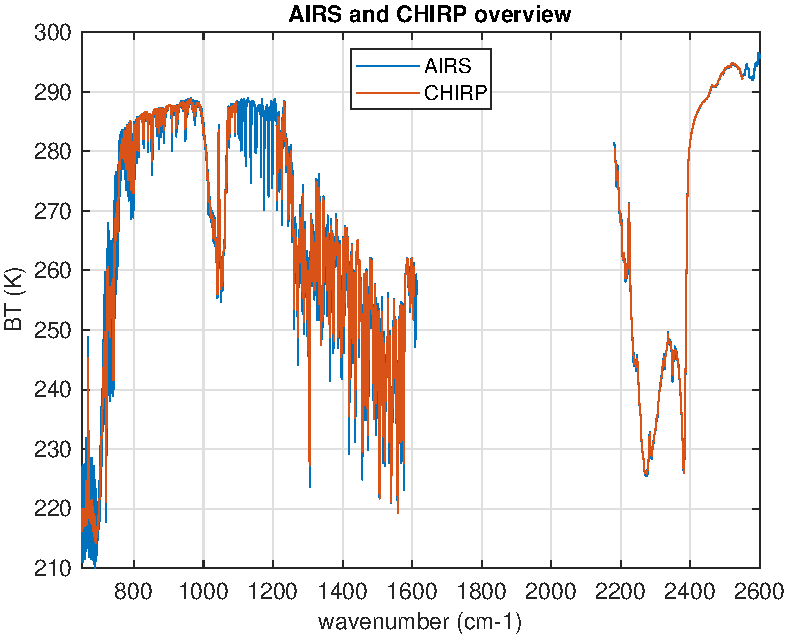
\includegraphics[width=\textwidth]{figures/airs_and_chirp_overview.pdf}
    \caption{Sample AIRS and AIRS-parent CHIRP spectra, granule means
      for 19 Aug 2018 granule 25.  The CHIRP bands are the intersection
      of the AIRS and CrIS bands.}
    \label{fig1}
  \end{minipage}\hfill
  \begin{minipage}[t]{0.45\textwidth}
    \centering
    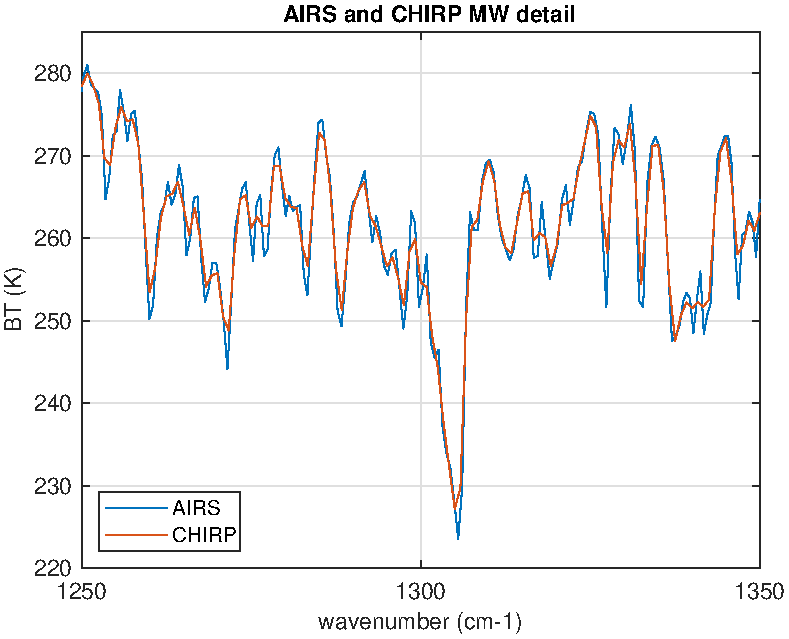
\includegraphics[width=\textwidth]{figures/airs_and_chirp_mw_detail.pdf}
    \caption{MW detail from the same granule.  Note that the data
      are on two different grids, and what we mainly see is the
      effect of the CHIRP apodization.}
    \label{fig2}
  \end{minipage}
\end{figure}

% CHIRP ILS
\begin{figure} % source a2cris_srfs.m
  \centering
  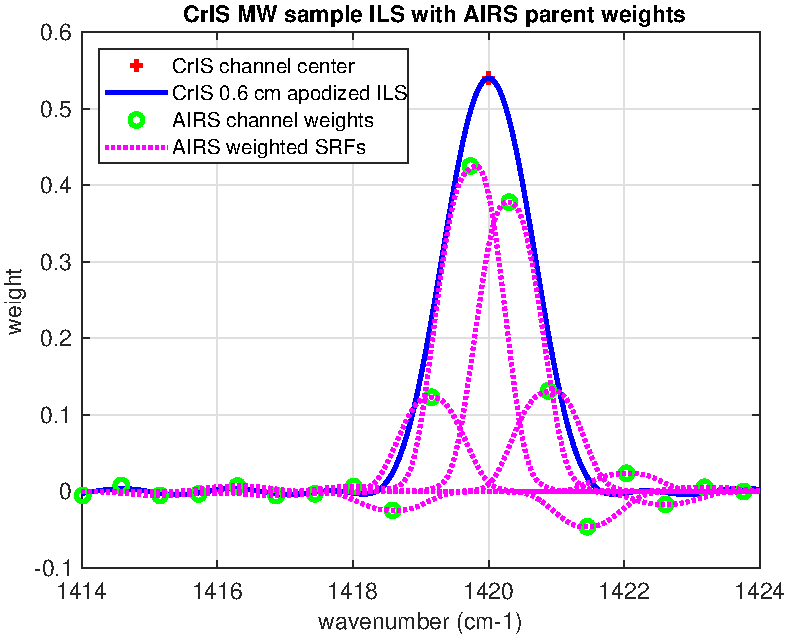
\includegraphics[height=9cm]{figures/sample_CrIS_ILS_with_AIRS_parent_SRFs.pdf}
  \caption{The MW CHIRP apodized ILS, together with weights for the
    AIRS channels, for the CHIRP channel shown.  The AIRS weights
    are paired with the corresponding AIRS SRFs, normalized to the
    weight values.}
  \label{fig3}
\end{figure}

For a long-term record we need radiance data in a single format---a
single frequency grid with a common ILS, and to the extent possible,
similar NEdN.  CHIRP radiances are for a nominal 3-band
interferometer with an {\opd} of $0.8$ {\cm} in the long-wave (LW),
$0.6$ {\cm} in the medium-wave (MW), and $0.4$ {\cm} in the
short-wave (SW) bands, with Hamming apodization applied to each band.
The MW and SW resolutions are lower than the CrIS-parent FSR {\opd}
of $0.8$ {\cm}, and were chosen to to give an approximate match to
the AIRS resolution for those bands.  Figure \ref{fig1} shows
typical AIRS and AIRS-parent CHIRP BT spectra, the granule means for
19 Aug 2018 granule 25.  The CHIRP bands are the intersection of the
AIRS and CrIS bands.  Figure \ref{fig2} is a MW detail from Figure
\ref{fig1}.  Note that the AIRS and CHIRP data are on two different
grids, and what we mainly see is the effect of the CHIRP
apodization.

For CrIS-parent CHIRP, we interpolate the CrIS Full Spectral
Resolution (FSR) product, with an $0.8$ {\cm} {\opd} for all three
bands, to the CHIRP grid, and then apply Hamming apodization.  The
CrIS-parent CHIRP ILS is then a Hamming-apodized sinc for a $0.8$
{\cm} {\opd} in the LW, $0.6$ {\cm} in the MW, and $0.4$ {\cm} in
the SW.  Figure \ref{fig3} shows this ILS for a typical CHIRP MW
channel.

We want to match this ILS for the AIRS-parent data.  But AIRS is a
grating spectrometer with a distinct response function for each
channel, while CrIS is a Michelson interferometer with a sinc
response function after calibration and corrections.  We use our
detailed knowledge of the AIRS spectral response functions to
deconvolve AIRS channel radiances to a resolution enhanced
intermediate representation.  This is done by taking a Moore-Penrose
pseudo-inverse of the tabulated AIRS SRFs and applying this to the
AIRS radiances, giving us deconvolved data at a $0.1$ {\wn} grid.
This is then reconvolved to the CHIRP user grid via resampling or
double Fourier interpolation.  The resulting translation can be
shown to be more accurate than more conventional interpolation or
regression \cite{mott2018}.  Figure \ref{fig3} includes the AIRS
channel weights and corresponding AIRS SRFs, normalized to the weight
values, for AIRS-parent data for this channel.  The weights are from
a row of a linearized approximation of the AIRS to CHIRP translation.

Hamming apodization (as mentioned above) and an optional bias
correction are applied to both translations.  Currently AIRS and
CrIS J1 parent are adjusted to match CrIS SNPP \cite{strow2021a}.
After translation from CrIS, the three bands have 713, 649, and 317
channels, respectively.  These are concatenated for the CHIRP
product, for a total of 1679 channels.  The CHIRP user grid does not
have a constant step size, the frequency steps are $1/(2 \,\opd)$.
The CHIRP field \texttt{wnum} is a 1679-vector which gives channel
frequencies, and \texttt{rad} is a 1679 by 12150 array of radiance
data.  AIRS-parent CHIRP uses the same channel set.  However the
AIRS-to-CHIRP translation gives only 1483 channels, due to slightly
different band spans.  These are embedded in the 1679 channel set,
with missing channels flagged as described in section \ref{qcnedn}.

%----------- section --------------------------------------------------%
\section{Sampling}
\label{sampling}

% one day track map
\begin{figure} % source plot_subpt.m
  \centering
  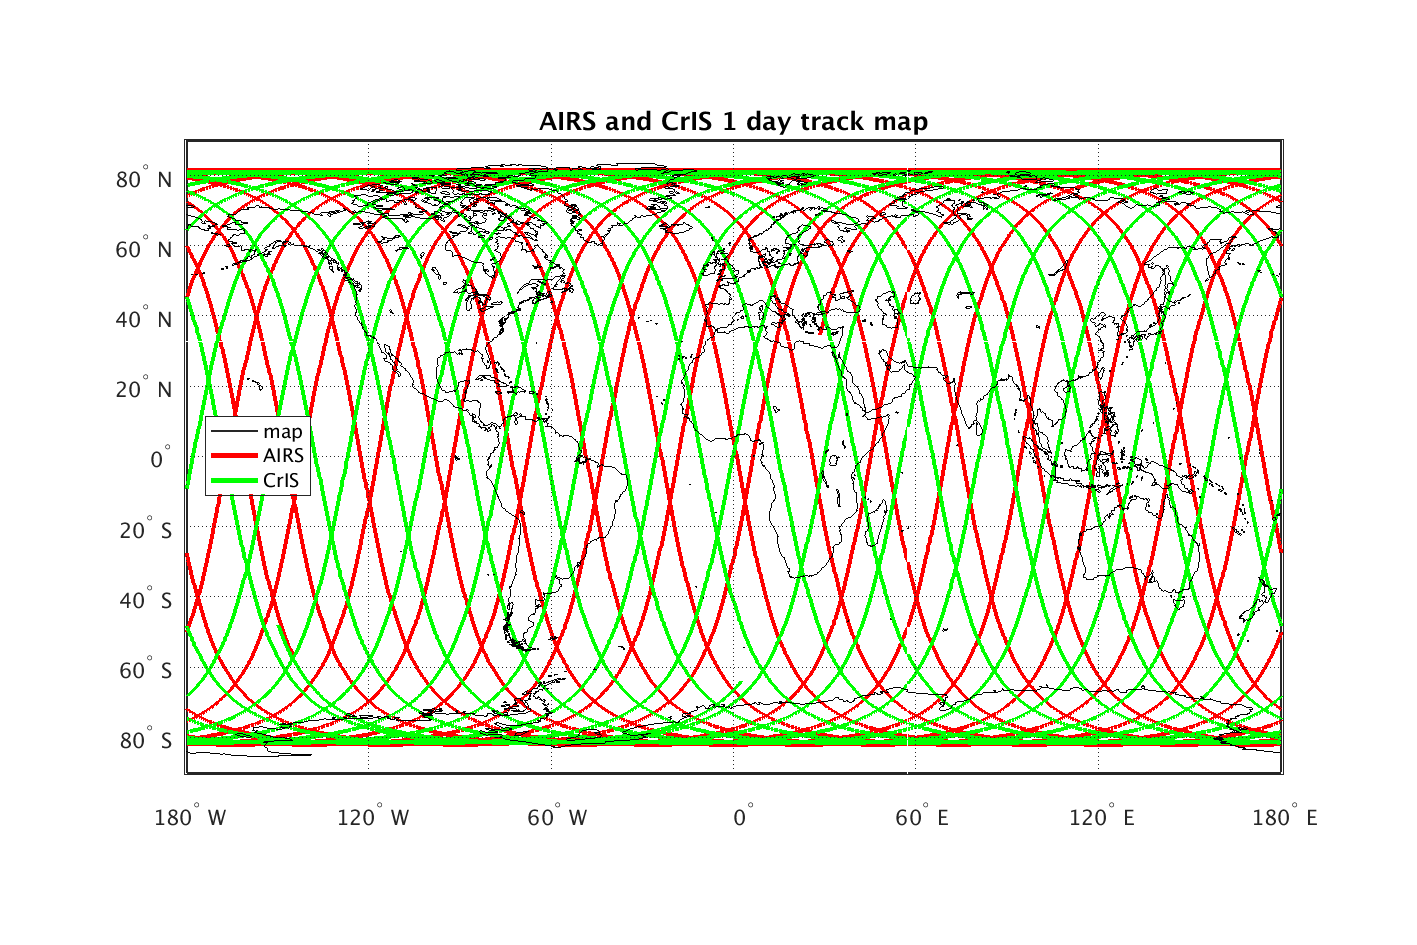
\includegraphics[height=10cm]{figures/subpt_1_day_all.png}
  \vskip-12mm
  \caption{Global one-day subpoint track map.}
  \label{fig4}
\end{figure}

% 16 day track maps
\begin{figure} % source plot_subpt.m
  \centering
  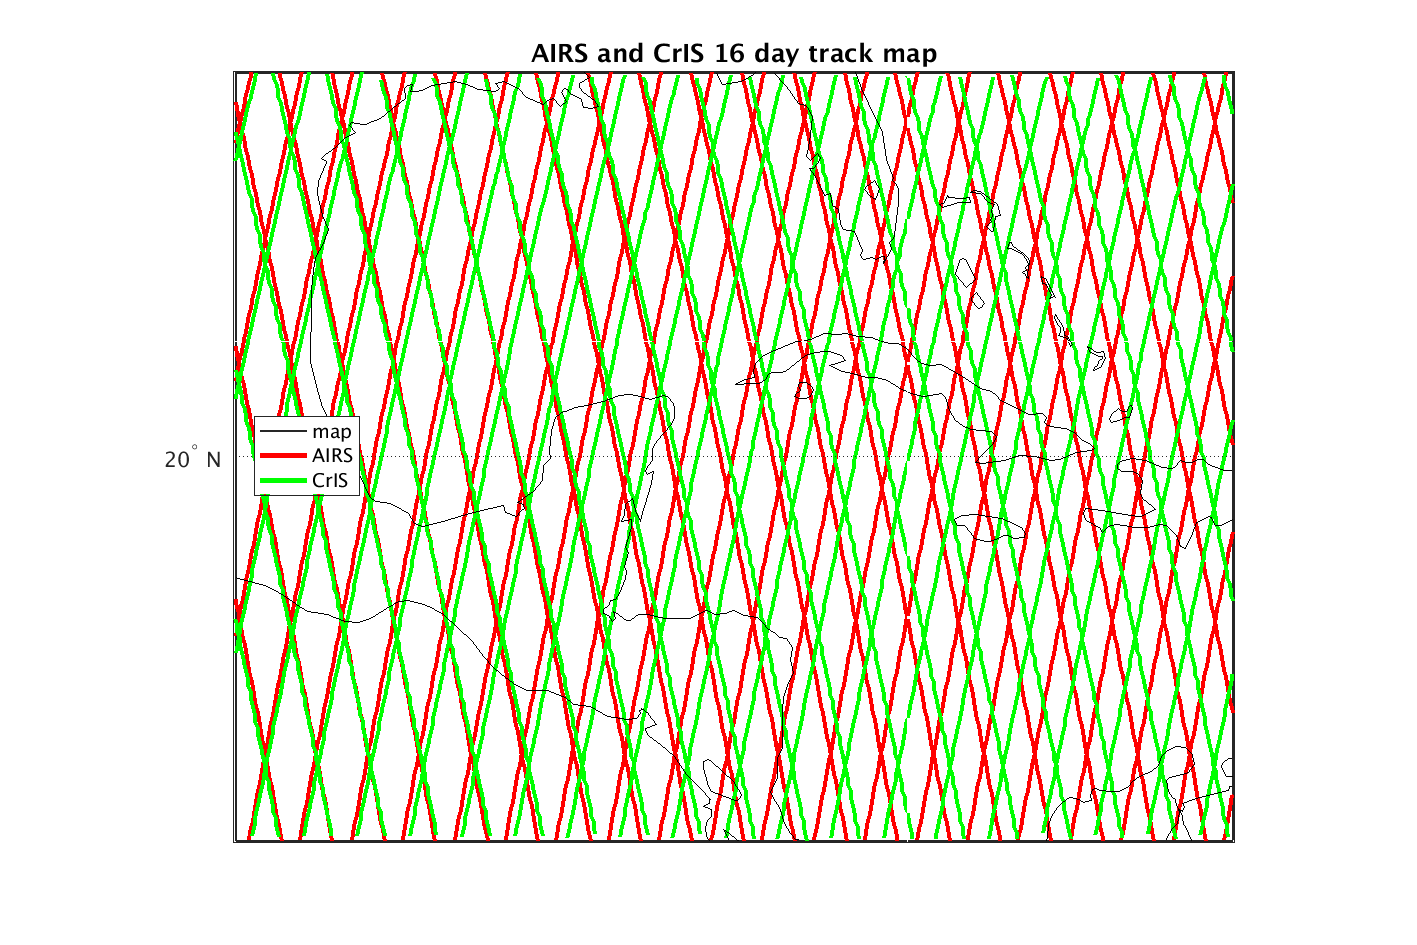
\includegraphics[height=10cm]{figures/subpt_16_day_zoom.png}
  \vskip-9mm
  \caption{Sixteen day subpoint track map for the Caribbean.}
  \label{fig5}
\end{figure}

% AIRS and CrIS secant of zenith angles
\begin{figure} % source plot_tbin.m
  \centering
  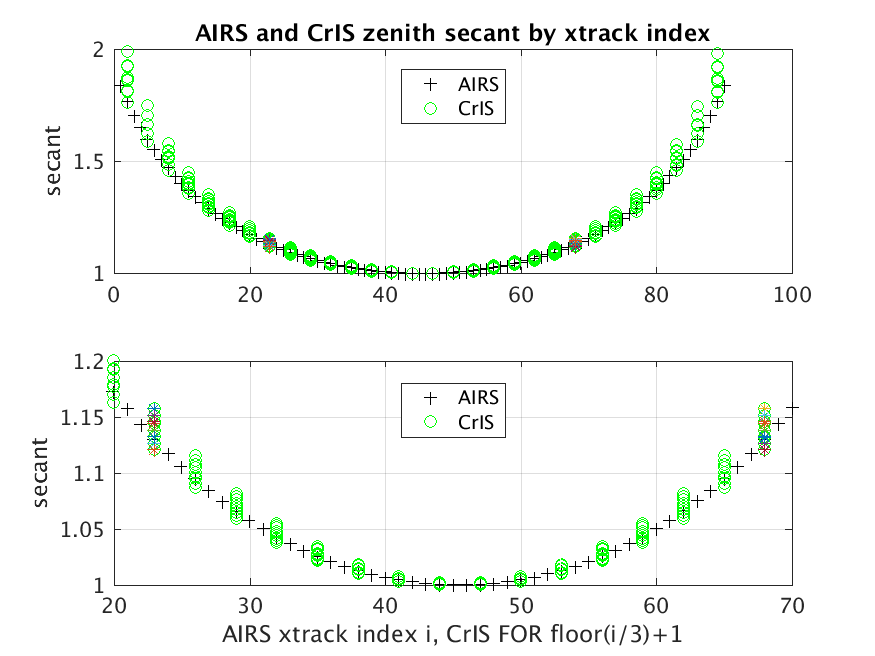
\includegraphics[height=10cm]{figures/AIRS_CrIS_secant_by_xtrack.png}
  \caption{AIRS and CrIS secant of zenith angles}
  \label{fig6}
\end{figure}

% CrIS Scans, from NOAA User Guide
\begin{figure} % source plot_tbin.m
  \centering
  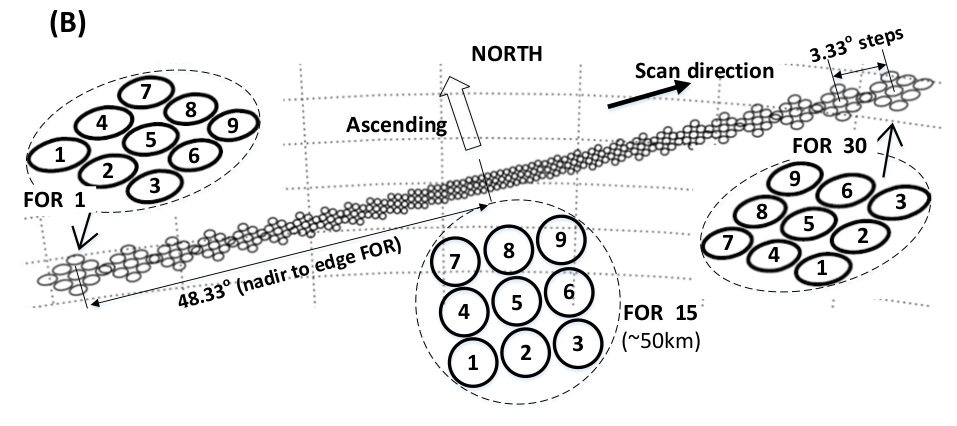
\includegraphics[width=0.9\linewidth]{figures/cris_for_2.png}
  \caption{CrIS scan geometry, from the NOAA User's Guide \cite{ntech1}}
  \label{fig7}
\end{figure}

AIRS and CrIS spatial sampling are similar, but not identical.
AIRS and CrIS are both in sun-synchronous polar orbits.  The CrIS
orbital period is 101.5 minutes, giving 227 orbits every 16 days.
The AIRS orbital period 98.8 minutes, giving 233 orbits every 16
days.  Note that 227 and 233 are both prime; there are no common
factors and so no repeating subpatterns.  Figure \ref{fig4} shows
global values for satellite subpoint for one day of AIRS and CrIS
data, and figure \ref{fig5} for 16 days, the full period before any
repeated positions, for the Caribbean.  AIRS and CrIS are
cross-track scanners, and in addition to subpoint tracks we want to
compare the scan geometry.  Figure \ref{fig6} shows the secant of
zenith angles for AIRS and CrIS.  The upper plot is for the full
scan widths, while the lower is a near-nadir detail.  The general
agreement is quite good, and the main difference we see is due to
the CrIS FOV grouping.

The AIRS L1c scan geometry is organized as 90 cross-track by 135
along-track observations, giving $90 \times 135 = 12150$ obs per
granule.  The CrIS L1b scan geometry is organized as 9 FOVs arranged
in a $3 \times 3$ field of regard (FOR), giving 9 simultaneous
observations.  There are 30 cross-track FOR looks and 45 along-track
FOR steps.  So again we have $9 \times 30 \times 45 = 12150$ obs per
granule.  Figure \ref{fig7} shows the relationship of the CrIS FOVs
and FOR as the scan moves from nadir to limb.  Note that the FOVs
rotate withing the FOR as we move toward the limbs.  CHIRP provides
both AIRS- and CrIS-style indexing, the AIRS-style indexing in the
fields \texttt{airs\_xtrack} and \texttt{airs\_atrack}, and
CrIS-style indexing, where xtrack and atrack are FOR rather than FOV
indices, in the fields \texttt{xtrack}, \texttt{atrack} and
\texttt{fov\_num}.  However due to the FOR rotation, we can't treat
the CrIS-parent data as a simple cross-track by along-track grid, as
with the AIRS-parent, for example for imaging.


%----------- section --------------------------------------------------%
\section{Quality Control and NEdN Estimates}
\label{qcnedn}

CHIRP Quality Control (QC) is straightforward.  There are two QC
fields per granule, \texttt{rad\_qc}, a 12150-vector with one flag
per obs, and \texttt{chan\_qc}, a 1679-vector with one flag per
channel.  For both vectors, 0 = OK, 1 = warn, and 2 = bad.  For
CrIS-parent CHIRP these fields are a summary of the parent product
state.  For AIRS-parent CHIRP the situation is more complex, due to
a significant and variable number of AIRS synthetic channels, and
because the set of 1483 channels from the AIRS translation are a
subset of the 1679 channels from the CrIS translation.

\subsection{AIRS-parent CHIRP QC}

For AIRS-parent CHIRP the 1679-element vector \texttt{chan\_qc} is
set to 2 (bad) for those channels that are not part of the 1483
channel set, as translated from AIRS.  This is a compromise that
give us a single frequency grid for CHIRP, regardless of the parent
sounder.  If we begin by choosing a set of channels to work with
AIRS-parent data, we can continue using that set with the change to
CrIS-parent, with no changes in our indexing.  In addition to
flagging missing channels, \texttt{chan\_qc} is set to 1 (warn) for
the six channels at the translation band edges, and when the
synthetic component exceeds a threshold, as described below.

The 12150-element vector \texttt{rad\_qc} has a flag for each obs.
These are set to 0 (OK) if the L1c field \texttt{instrument\_state}
is OK and radiance and geo values pass some basic sanity checks.
\texttt{rad\_qc} is always 0 or 2 for AIRS-parent CHIRP, because
AIRS L1c doesn't have a warn flag.

\subsection{AIRS Synthetic Channels}

As an alternative to a warn flag, and to fill band gaps, AIRS L1c
provides synthetic values for some observations and channels.  That
is, for a particular observation---a radiance vector with an
associated time, geolocation, and support data---some of the
channels may be synthetic.  Some of these channels are synthetic
only occasionally, others more frequently, and some are always
synthetic.  These synthetic channels are flagged in the L1c file,
for every observation and channel.  In addition, the granule file
has a per-granule summary, L1cNumSynth, for each L1c channel.  This
is the number of times the channel was filled with a synthetic
value.  L1cNumSynth can range from zero, for no synthetic values, to
12150, for all synthetic.  Figure \ref{fig8} shows the sum of all
synthetic values by channel, for 5036 consecutive AIRS granules,
approximately 21 days of data.  Counts are shown on a log scale.
Figure \ref{fig9} shows the same data as synthetic values per
channel, sorted by number of synthetic values.  This shows the wide
range of values, from few or no synthetic values for some channels,
to entirely synthetic values for others.

For some applications we may not want a significant synthetic
component.  The CHIRP field \texttt{synth\_frac} provides the AIRS
synthetic component for each CHIRP channel.  This can range from
zero, for no synthetic component, to one, for entirely synthetic.
To get this value we linearize the AIRS to CrIS translation and
apply it to the AIRS L1cNumSynth, to get a corresponding NumSynth
value for CHIRP.  This is normalized as a fraction and becomes the
CHIRP field \texttt{synth\_frac}.  Figure \ref{fig10} shows the
AIRS-parent CHIRP synthetic fraction for a single representative
granule. This can be used to select channels with a relatively small
synthetic component.  Figure \ref{fig11} show the AIRS-parent CHIRP
synthetic fraction, sorted by synthetic fraction magnitude.  This
shows the variability of \texttt{synth\_frac}.  If
$\hbox{\texttt{synth\_frac}} > 0.25$, we set \texttt{chan\_qc} to
warn.

% The threshold $0.25$ is a parameter that can be changed in the
% production YAML specs.

\begin{figure}
  \centering
  \begin{minipage}[t]{0.45\textwidth}
    \centering
    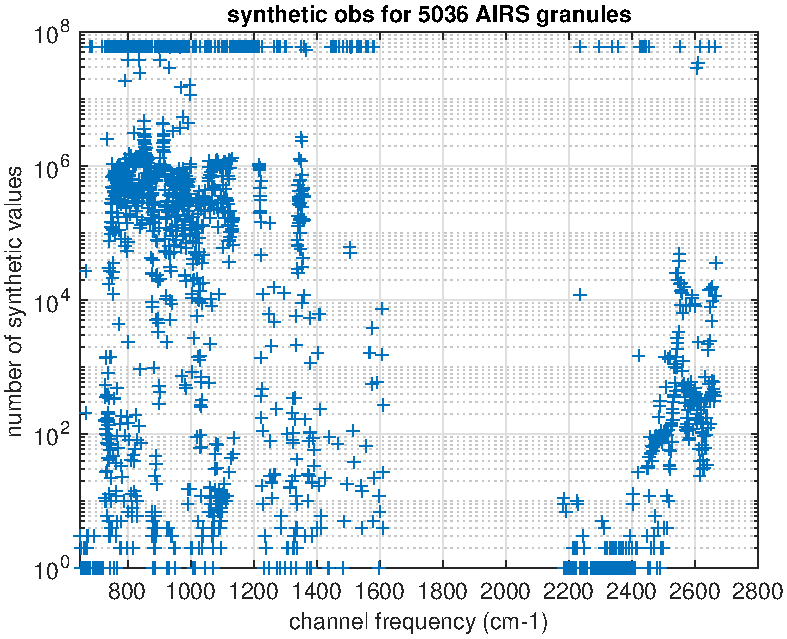
\includegraphics[width=\textwidth]{figures/synth_obs_freq_order.pdf}
    \caption{The sum of synthetic values by channel for 5036 AIRS
      granules.  Counts are on a log scale.}
    \label{fig8}
  \end{minipage}\hfill
  \begin{minipage}[t]{0.45\textwidth}
    \centering
    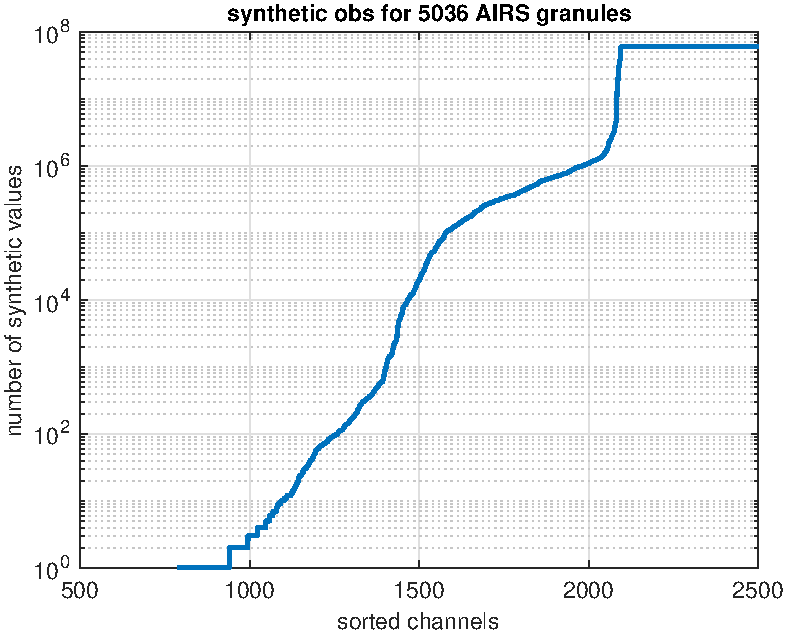
\includegraphics[width=\textwidth]{figures/synthetic_obs_counts.pdf}
    \caption{Synthetic values per channel, sorted by number of
      synthetic values.  This shows the range of these values.}
    \label{fig9}
  \end{minipage}
\end{figure}

\begin{figure}
  \centering
  \begin{minipage}{0.45\textwidth}
    \centering
    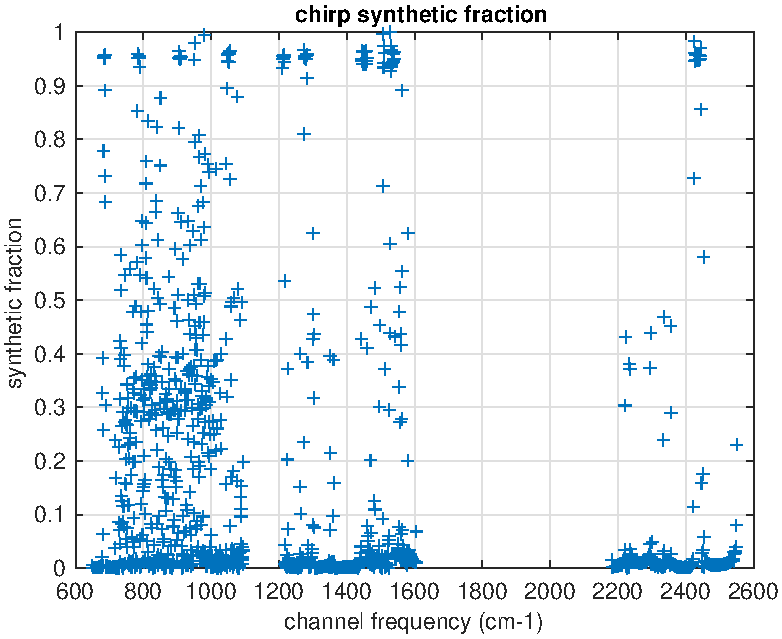
\includegraphics[width=\textwidth]{figures/chirp_sample_syn_frac.pdf}
    \caption{AIRS-parent CHIRP synthetic fraction for a single
      representative granule.  This can be used to select channels
      with a relatively small synthetic component.}
    \label{fig10}
  \end{minipage}\hfill
  \begin{minipage}{0.45\textwidth}
    \centering
    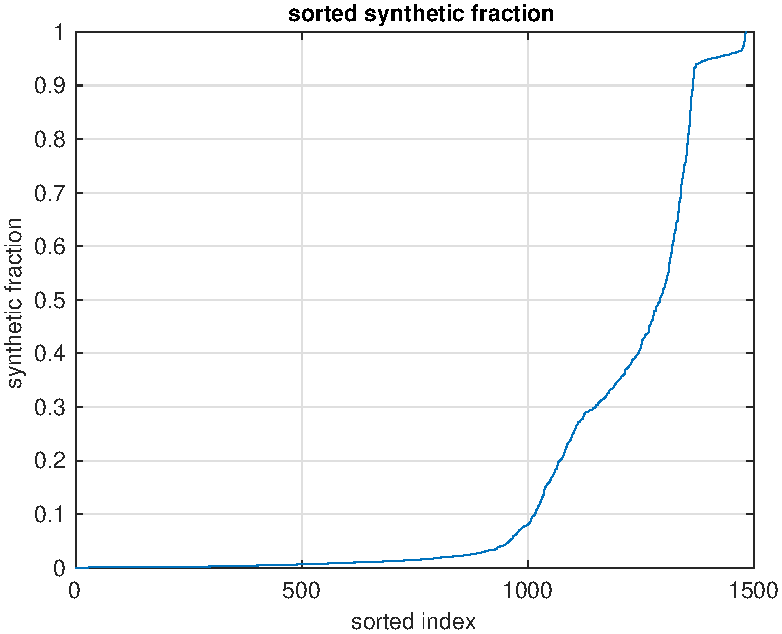
\includegraphics[width=\textwidth]{figures/chirp_sorted_syn_frac.pdf}
    \caption{AIRS-parent CHIRP synthetic fraction, sorted by
      synthetic fraction magnitude.  This shows the variability of
      synth\_frac.}
    \label{fig11}
  \end{minipage}
\end{figure}

\begin{figure}
  \centering
  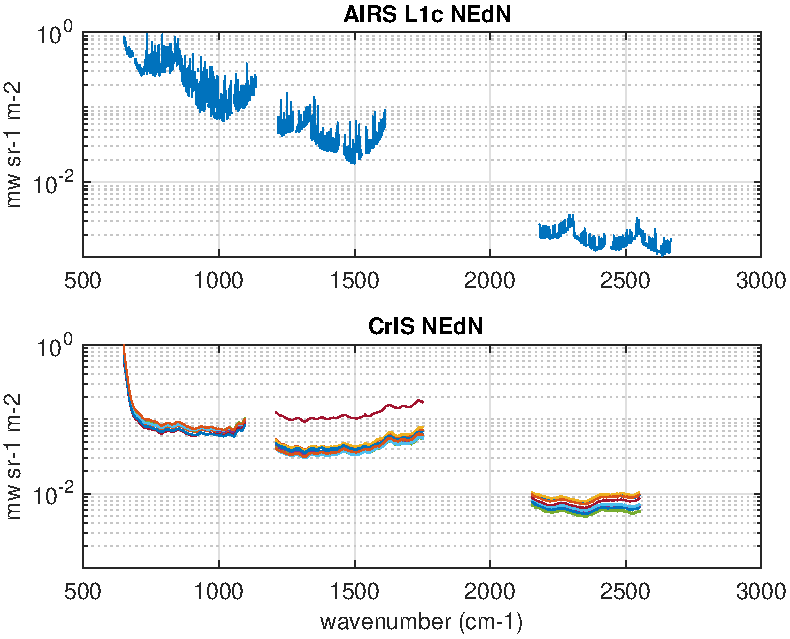
\includegraphics[height=10cm]{figures/sample_airs_and_cris_nedn.pdf}
  \caption{Sample AIRS and CrIS {\nedn} for 2018 doy 231 granules 25
    and 21, two relatively warm granules.}
  \label{fig12}
\end{figure}

\begin{figure}
  \centering
  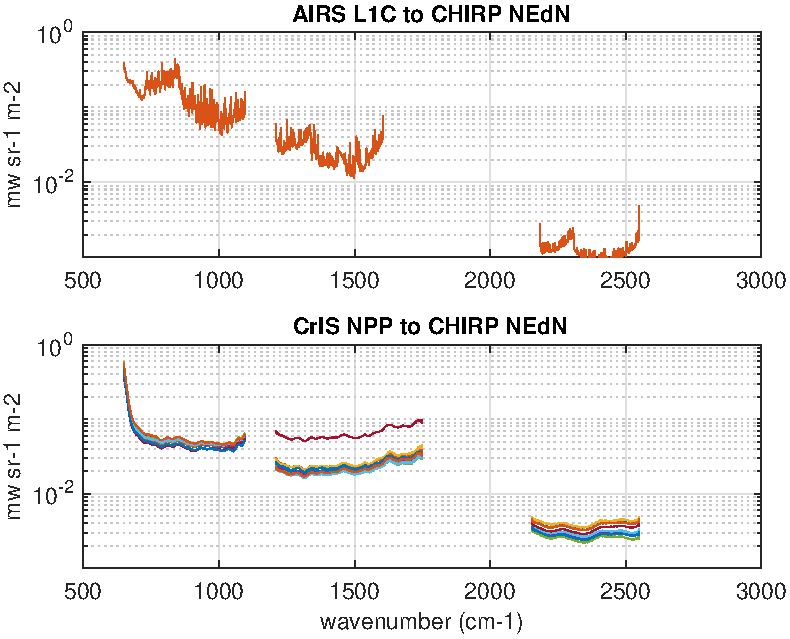
\includegraphics[height=10cm]{figures/chirp_nedn_from_airs_and_cris.pdf}
  \caption{Sample CHIRP {\nedn} for AIRS and CrIS parent data, for
    the granules shown in figure \ref{fig12}.  The noise is
    significantly less for the translations.}
  \label{fig13}
\end{figure}

\subsection{AIRS-parent CHIRP NEdN}

To find {\nedn} for AIRS-parent CHIRP, we start with an AIRS L1c
{\nedn} estimate.  Unfortunately the synthetic obs do not include
values for {\nedn}.  As a compromise we take the mean of valid
{\nedn} values over an AIRS granule and interpolate over the gaps
for the synthetic channels.  Given the AIRS estimate, we add
Gaussian noise at the AIRS {\nedn} to a black-body spectra at 280K,
do the translation, and measure the resulting noise.  This is done
repeatedly and the mean of the measurement is reported.  Details are
described in \cite{mott2018}.  The correlated fraction of AIRS noise
varies from module to module, and is significant for some modules.
The translation will preserve this correlation.  {\nedn} estimates
for this case are a matter for future work.

Figure \ref{fig12} shows typical values for AIRS and CrIS {\nedn}
for 2018 doy 231 granules 25 and 21, respectively; two relatively
warm granules.  Figure \ref{fig13} shows the corresponding CHIRP
{\nedn} for AIRS and CrIS parent data, for the same granules.
The noise is significantly less for the translation.  This to be
expected since both apodization and down-interpolation reduce noise.

\subsection{CrIS-parent CHIRP QC and NEdN}

In contrast with AIRS, CrIS-parent CHIRP QC and {\nedn} are
relatively simple.  CrIS-parent CHIRP QC is determined from the CrIS
parent, by combining the fields for the individual CrIS bands.
\texttt{chan\_qc} is set to 0 (OK) for CrIS-parent CHIRP.  Possibly
we should set \texttt{chan\_qc} to warn at the band edges, as we do
for AIRS parent, but we are not doing this now.  CrIS-parent CHIRP
{\nedn} is derived from the high res CrIS {\nedn} with scale factors
to take into account the interpolation and apodization.  These are
\begin{itemize}
   \item LW, 0.6325, for Hamming apodization only
   \item MW, 0.5455, for interpolation and Hamming apodization
   \item SW, 0.4446, for interpolation and Hamming apodization
\end{itemize}

%----------- section --------------------------------------------------%
\section{Further Information on CHIRP}
Further information and help on using CHIRP, beyond what is discussed
below, can be found at
\href{https://infraredclimate.org}{https://infraredclimate.org}, or send
email to
\href{mailto:chirp@infraredclimate.org}{chirp@infraredclimate.org}.  This
web site will also contain information on the Level 1b products produced at
GES-DIS for the series of CrIS instruments, starting with SNPP-CrIS and
continued with the JPSS series of CrIS instruments.

%----------- section --------------------------------------------------%
\bibliographystyle{abbrv}
\bibliography{user_guide}

\appendix
\section{Acronyms}

\begin{center}
\begin{tabular}{ m{2cm} m{10cm} }
AIRS    & Atmospheric Infrared Sounder \\
CHIRP   & Combined Hyperspectral Infrared Radiance Product \\
CrIS    & Cross-track Infrared Sounder \\
DISC    & Data and Information Services Center \\
FOV     & Field of View \\
FOR     & Field of Regard \\
FSR     & Full Spectral Resolution \\
GSFC    & Goddard Spaceflight Center \\
ILS     & Instrument Line Shape \\
IASI    & Infrared Atmospheric Sounding Interferometer \\
JPSS    & Joint Polar Satellite System \\
LW      & Long-Wave \\
MW      & Mid-Wave \\
SW      & Short-Wave \\
NASA    & National Aeronautics and Space Administration \\
NOAA    & National Oceanic and Atmospheric Administration \\
NEdN    & Noise Equivalent Differential Radiance \\
QC      & Quality Control \\
SIPS    & Science Investigator-led Processing System \\
SNPP    & Suomi-National Polar-Orbiting Preparatory Project \\
SRF     & Spectral Response Function \\
STAR    & Center for Satellite Applications and Research \\
\end{tabular}
\end{center}

\section{Filename Conventions}

CHIRP granule filenames are divided into fields separated by a dot
character.  This is best illustrated by example.  The following are
typical granule file names for AIRS AQUA, CrIS SNPP, and CrIS J1
(aka NOAA-20).

\begin{center}
\texttt{SNDR.SS1330.CHIRP.20180901T1835.m06.g186.L1\_AQ.std.v02\_20.U.201219110001.nc} \\
\texttt{SNDR.SS1330.CHIRP.20180821T0129.m06.g016.L1\_SN.std.v02\_20.U.200917211403.nc} \\
\texttt{SNDR.SS1330.CHIRP.20180913T2217.m06.g224.L1\_J1.std.v02\_20.U.201215180423.nc} \\
\texttt{~~1~~~~~2~~~~~3~~~~~~~~4~~~~~~~~~5~~~~6~~~~7~~~~8~~~~9~~~10~~~~~~11~~~~~12} \\
\end{center}

The 12 fields correspond to CHIRP attributes, and are defined in the
table below.  Field 7, the \texttt{product\_name\_type\_id}, is of
particular interest.  The sub-fields AQ, SN, and J1 are two letter
codes for AIRS AQUA, CrIS Sunomi NPP, and CrIS J1 (aka NOAA-20),
respectively.  This is the parent sounder for the granule.  A suffix
``CAL'', for example L1\_AQ\_CAL, L1\_NP\_CAL, or L1\_J1\_CAL,
indicates a support product, while no suffix (as in the examples
above) indicates the primary CHIRP product.

{\footnotesize
\begin{center}
\begin{tabular}{|m{7mm}|m{5.5cm}|m{8cm}| }
  \hline
  Field & Attribute Name & Comment \\
  \hline\hline
   1 & \texttt{product\_name\_project} & Always ``SNDR'', for Sounder
   SIPS \\
   \hline
   2 & \texttt{product\_name\_platform} & Always ``SS1330'', a virtual
   platform in a 13:30 Sun-Synchronous polar orbit\\
   \hline
   3 & \texttt{product\_name\_instr} & Always “CHIRP” \\
   \hline
   4 & \texttt{gran\_id} & Granule start time \\
   \hline
   5 & \texttt{product\_name\_duration} & Always ``m06'' meaning 6
   minutes \\
   \hline
   6 & \texttt{product\_name\_granule\_number} & Granule number from
   g001 – g240 \\
   \hline
   7 & \texttt{product\_name\_type\_id} & ``L1\_'' + PL [+
     ``\_CAL''], where PL platform code can be ``AQ'', ``SN'', or
   ``J1''.  The optional tag ``\_CAL'' marks redundant calibration
   data, not considered part of the main CHIRP product. \\
   \hline
   8 & \texttt{product\_name\_variant} & Always ``std''\\
   \hline
   9 & \texttt{product\_name\_version} & For example ``V02\_48'' for
   version 02.48 \\
   \hline
   10 & \texttt{product\_name\_producer} & ``G'' for data produced by NASA GSFC\\
   \hline
   11 & \texttt{product\_name\_timestamp} & Processing timestamp \\
   \hline
   12 & \texttt{product\_name\_extension} & Always ``.nc'' \\
   \hline
\end{tabular}
\end{center}
}

% small sizes: \tiny \scriptsize \footnotesize \small

\section{Field Definitions}
\label{fields}
{\footnotesize

\subsection{Dimensions}

\begin{center}
\begin{xltabular}{\textwidth}{|l|l|m{10cm}|}

% >{\hsize=10\hsize\linewidth=\hsize}X|
% }

\hline
Name & Size & Description\tabularnewline\hline
\hline
fov & 9 & Field-of-view dimension\tabularnewline\hline
obs & 12,150 & number of spectra in 6-minute L1 CHIRP for the 13:30
orbit. 135*90 or 45*30*9\tabularnewline\hline
wnum & 1,679 & IR channel number\tabularnewline\hline
fov\_poly & 8 & lat\_bnds, lon\_bnds points defining the polygon
bounding an FOV (anticlockwise as viewed from above)\tabularnewline\hline
utc\_tuple & 8 & parts of UTC time: year, month, day, hour, minute,
second, millisec, microsec\tabularnewline\hline

\end{xltabular}
\end{center}

}
{\scriptsize

\subsection{Variables}

\begin{center}
\begin{xltabular}{\textwidth}{|l|l|
>{\hsize=.4\hsize\linewidth=\hsize}X|
>{\hsize=2\hsize\linewidth=\hsize}X|
>{\hsize=.6\hsize\linewidth=\hsize}X|
l|
}

\hline
Name & Type & Dim & Description & Units & Ancillary 
\tabularnewline\hline\hline
obs\_id & string & obs & unique earth view observation identifier. &
&\tabularnewline\hline
obs\_time\_tai93 & double & obs & earth view observation midtime for
each FOV & seconds since 1993-01-01 00:00 & \tabularnewline\hline
obs\_time\_utc & uint16 & obs, utc\_tuple & UTC earth view observation
time as an array of integers: year, month, day, hour, minute, second,
millisec, microsec & &\tabularnewline\hline
lat & float & obs & latitude of FOV center & degrees\_north &
bnds\tabularnewline\hline
lon & float & obs & longitude of FOV center & degrees\_east &
bnds\tabularnewline\hline
land\_frac & float & obs & land fraction over the FOV & unitless
&\tabularnewline\hline
surf\_alt & float & obs & mean surface altitude wrt earth model over the
FOV & m &\tabularnewline\hline
surf\_alt\_sdev & float & obs & standard deviation of surface altitude
within the FOV & m &\tabularnewline\hline
sun\_glint\_lat & float & obs & sun glint spot latitude at
scan\_mid\_time. Fill for night observations. & degrees\_north
&\tabularnewline\hline
sun\_glint\_lon & float & obs & sun glint spot longitude at
scan\_mid\_time. Fill for night observations. & degrees\_east
&\tabularnewline\hline
sol\_zen & float & obs & solar zenith angle at the center of the FOV &
degree &\tabularnewline\hline
sol\_azi & float & obs & solar azimuth angle at the center of the FOV
(clockwise from North) & degree &\tabularnewline\hline
sun\_glint\_dist & float & obs & Distance from the center of the
calculated sun glint spot to the center of the spot. Note that there may
not be a glint for cloudy or land cases and in ocean cases the glint can
move based on wind conditions. Fill for night observations. & m
&\tabularnewline\hline
view\_ang & float & obs & off nadir pointing angle & degree
&\tabularnewline\hline
sat\_zen & float & obs & satellite zenith angle at the center of the FOV
& degree &\tabularnewline\hline
sat\_azi & float & obs & satellite azimuth angle at the center of the
FOV (clockwise from North) & degree &\tabularnewline\hline
sat\_range & float & obs & line of sight distance between satellite and
FOV center & m &\tabularnewline\hline
asc\_flag & ubyte & obs & ascending orbit flag: 1 if ascending, 0
descending & &\tabularnewline\hline
subsat\_lat & float & obs & sub-satellite latitude at scan\_mid\_time &
degrees\_north &\tabularnewline\hline
subsat\_lon & float & obs & sub-satellite longitude at scan\_mid\_time &
degrees\_east &\tabularnewline\hline
scan\_mid\_time & double & obs & TAI93 at middle of earth scene scans &
seconds since 1993-01-01 00:00 &\tabularnewline\hline
sat\_alt & float & obs & satellite altitude with respect to earth model
at scan\_mid\_time & m &\tabularnewline\hline
local\_solar\_time & float & obs & local apparent solar time in hours
from midnight & hours &\tabularnewline\hline
utc\_tuple\_lbl & string & utc\_tuple & names of the elements of UTC
when it is expressed as an array of integers
year, month, day, hour, minute, second, millisecond, microsecond &
&\tabularnewline\hline
rad & float32 & obs, wnum & spectral radiance & mW/(m2 sr cm-1) & 
qc\tabularnewline\hline
synth\_frac & float32 & wnum & File mean fraction of signal that is
attributed to synthesized AIRS Level-1C values & unitless
&\tabularnewline\hline
nedn & float32 & fov, wnum & noise equivalent differential radiance &
mW/(m2 sr cm-1) &\tabularnewline\hline
atrack & ubyte & obs & Along-track index of Field Of Regard & unitless
&\tabularnewline\hline
xtrack & ubyte & obs & Cross-track index of Field Of Regard & unitless &
\tabularnewline\hline
fov\_num & ubyte & obs & Field Of View number in FOR & unitless
&\tabularnewline\hline
airs\_atrack & ubyte & obs & AIRS-like along-track index of Field Of
View & unitless &\tabularnewline\hline
airs\_xtrack & ubyte & obs & AIRS-like cross-track index of Field Of
View & unitless &\tabularnewline\hline
wnum & float64 & wnum & wavenumber & cm-1 & \tabularnewline
\hline
\end{xltabular}
\end{center}



\subsection{Attributes}
\label{attrs}

\begin{center}
\begin{xltabular}{1.1\textwidth}{|m{4cm}|l|l|
>{\hsize=12\hsize\linewidth=\hsize}X|
>{\hsize=18\hsize\linewidth=\hsize}X|
}

\hline
Name & Type & Size & Value & Description\tabularnewline\hline
\hline
keywords & string & 1 & EARTH SCIENCE,
SPECTRAL ENGINEERING, INFRARED WAVELENGTHS,
INFRARED RADIANCE & A comma-separated list of key words and/or phrases.
Keywords may be common words or phrases, terms from a controlled
vocabulary (GCMD is often used), or URIs for terms from a controlled
vocabulary (see also "keywords\_vocabulary" attribute).\tabularnewline\hline
Conventions & string & 1 & CF-1.6, ACDD-1.3 & A
comma-separated list of the conventions that are followed by the
dataset.\tabularnewline\hline
history & string & 1 & & Provides an audit trail for modifications to
the original data. This attribute is also in the NetCDF Users Guide:
'This is a character array with a line for each invocation of a program
that has modified the dataset. Well-behaved generic netCDF applications
should append a line containing: date, time of day, user name, program
name and command arguments.' To include a more complete description you
can append a reference to an ISO Lineage entity; see NOAA EDM ISO
Lineage guidance.\tabularnewline\hline
source & string & 1 & AIRS and CrIS instrument telemetry & The method of
production of the original data. If it was model-generated, source
should name the model and its version. If it is observational, source
should characterize it. This attribute is defined in the CF Conventions.
Examples: 'temperature from CTD \#1234'; 'world model
v.0.1'.\tabularnewline\hline
processing\_level & string & 1 & 1 & A textual description of the
processing (or quality control) level of the data.\tabularnewline\hline
product\_name\_type\_id & string & 1 & L1 & Product name as it appears
in product\_name (L1A, L1B, L2, SNO\_AIRS\_CrIS)\tabularnewline\hline
comment & string & 1 & & Miscellaneous information about the data or
methods used to produce it. Can be empty.\tabularnewline\hline
acknowledgment & string & 1 & Support for this research was provided by
NASA. & A place to acknowledge various types of support for the project
that produced this data.\tabularnewline\hline
license & string & 1 & Limited to Sounder SIPS affiliates & Provide the
URL to a standard or specific license, enter "Freely Distributed" or
"None", or describe any restrictions to data access and distribution in
free text.\tabularnewline\hline
standard\_name\_vocabulary & string & 1 & CF Standard Name Table v28 &
The name and version of the controlled vocabulary from which variable
standard names are taken. (Values for any standard\_name attribute must
come from the CF Standard Names vocabulary for the data file or product
to comply with CF.) Example: 'CF Standard Name Table
v27'.\tabularnewline\hline
date\_created & string & 1 & Unassigned & The date on which this version
of the data was created. (Modification of values implies a new version,
hence this would be assigned the date of the most recent values
modification.) Metadata changes are not considered when assigning the
date\_created. The ISO 8601:2004 extended date format is recommended, as
described in the Attribute Content Guidance section.\tabularnewline\hline
creator\_name & string & 1 & Unassigned & The name of the person (or
other creator type specified by the creator\_type attribute) principally
responsible for creating this data.\tabularnewline\hline
creator\_email & string & 1 & Unassigned & The email address of the
person (or other creator type specified by the creator\_type attribute)
principally responsible for creating this data.\tabularnewline\hline
creator\_url & string & 1 & Unassigned & The URL of the person (or other
creator type specified by the creator\_type attribute) principally
responsible for creating this data.\tabularnewline\hline
institution & string & 1 & Unassigned & Processing facility that
produced this file\tabularnewline\hline
project & string & 1 & Sounder SIPS & The name of the project(s)
principally responsible for originating this data. Multiple projects can
be separated by commas, as described under Attribute Content Guidelines.
Examples: 'PATMOS-X', 'Extended Continental Shelf
Project'.\tabularnewline\hline
product\_name\_project & string & 1 & SNDR & The name of the project as
it appears in the file name. 'SNDR' for all Sounder SIPS products, even
AIRS products.\tabularnewline\hline
publisher\_name & string & 1 & Unassigned & The name of the person (or
other entity specified by the publisher\_type attribute) responsible for
publishing the data file or product to users, with its current metadata
and format.\tabularnewline\hline
publisher\_email & string & 1 & Unassigned & The email address of the
person (or other entity specified by the publisher\_type attribute)
responsible for publishing the data file or product to users, with its
current metadata and format.\tabularnewline\hline
publisher\_url & string & 1 & Unassigned & The URL of the person (or
other entity specified by the publisher\_type attribute) responsible for
publishing the data file or product to users, with its current metadata
and format.\tabularnewline\hline
geospatial\_bounds & string & 1 & & Describes the data's 2D or 3D
geospatial extent in OGC's Well-Known Text (WKT) Geometry format
(reference the OGC Simple Feature Access (SFA) specification). The
meaning and order of values for each point's coordinates depends on the
coordinate reference system (CRS). The ACDD default is 2D geometry in
the EPSG:4326 coordinate reference system. The default may be overridden
with geospatial\_bounds\_crs and geospatial\_bounds\_vertical\_crs (see
those attributes). EPSG:4326 coordinate values are longitude (decimal
degrees\_east) and latitude (decimal degrees\_north), in that order.
Longitude values in the default case are limited to the {[}-180, 180)
range. Example: 'POLYGON ((-111.29 40.26, -111.29 41.26, -110.29 41.26,
-110.29 40.26, -111.29 40.26))'.\tabularnewline\hline
geospatial\_bounds\_crs & string & 1 & EPSG:4326 & The coordinate
reference system (CRS) of the point coordinates in the
geospatial\_bounds attribute. This CRS may be 2-dimensional or
3-dimensional, but together with geospatial\_bounds\_vertical\_crs, if
that attribute is supplied, must match the dimensionality, order, and
meaning of point coordinate values in the geospatial\_bounds attribute.
If geospatial\_bounds\_vertical\_crs is also present then this attribute
must only specify a 2D CRS. EPSG CRSs are strongly recommended. If this
attribute is not specified, the CRS is assumed to be EPSG:4326.
Examples: 'EPSG:4979' (the 3D WGS84 CRS), 'EPSG:4047'.\tabularnewline\hline
geospatial\_lat\_min & float & 1 & 9.9692099683868690e+36f & Describes a
simple lower latitude limit; may be part of a 2- or 3-dimensional
bounding region. Geospatial\_lat\_min specifies the southernmost
latitude covered by the dataset.\tabularnewline\hline
geospatial\_lat\_max & float & 1 & 9.9692099683868690e+36f & Describes a
simple upper latitude limit; may be part of a 2- or 3-dimensional
bounding region. Geospatial\_lat\_max specifies the northernmost
latitude covered by the dataset.\tabularnewline\hline
geospatial\_lon\_min & float & 1 & 9.9692099683868690e+36f & Describes a
simple longitude limit; may be part of a 2- or 3-dimensional bounding
region. geospatial\_lon\_min specifies the westernmost longitude covered
by the dataset. See also geospatial\_lon\_max.\tabularnewline\hline
geospatial\_lon\_max & float & 1 & 9.9692099683868690e+36f & Describes a
simple longitude limit; may be part of a 2- or 3-dimensional bounding
region. geospatial\_lon\_max specifies the easternmost longitude covered
by the dataset. Cases where geospatial\_lon\_min is greater than
geospatial\_lon\_max indicate the bounding box extends from
geospatial\_lon\_max, through the longitude range discontinuity meridian
(either the antimeridian for -180:180 values, or Prime Meridian for
0:360 values), to geospatial\_lon\_min; for example,
geospatial\_lon\_min=170 and geospatial\_lon\_max=-175 incorporates 15
degrees of longitude (ranges 170 to 180 and -180 to
-175).\tabularnewline\hline
time\_coverage\_start & string & 1 & & Nominal start time. Describes the
time of the first data point in the data set. Use the ISO 8601:2004 date
format, preferably the extended format as recommended in the Attribute
Content Guidance section.\tabularnewline\hline
time\_of\_first\_valid\_obs & string & 1 & & Describes the time of the
first valid data point in the data set. Use the ISO 8601:2004 date
extended format.\tabularnewline\hline
time\_coverage\_mid & string & 1 & & Describes the midpoint between the
nominal start and end times. Use the ISO 8601:2004 date format,
preferably the extended format as recommended in the Attribute Content
Guidance section.\tabularnewline\hline
time\_coverage\_end & string & 1 & & Nominal end time. Describes the
time of the last data point in the data set. Use ISO 8601:2004 date
format, preferably the extended format as recommended in the Attribute
Content Guidance section.\tabularnewline\hline
time\_of\_last\_valid\_obs & string & 1 & & Describes the time of the
last valid data point in the data set. Use the ISO 8601:2004 date
extended format.\tabularnewline\hline
time\_coverage\_duration & string & 1 & P0000-00-00T00:06:00 & Describes
the duration of the data set. Use ISO 8601:2004 duration format,
preferably the extended format as recommended in the Attribute Content
Guidance section.\tabularnewline\hline
product\_name\_duration & string & 1 & m06 & Product duration as it
appears in product\_name (m06 means six minutes)\tabularnewline\hline
creator\_type & string & 1 & institution & Specifies type of creator
with one of the following: 'person', 'group', 'institution', or
'position'. If this attribute is not specified, the creator is assumed
to be a person.\tabularnewline\hline
creator\_institution & string & 1 & Jet Propulsion Laboratory -\/-
California Institute of Technology & The institution of the creator;
should uniquely identify the creator's institution. This attribute's
value should be specified even if it matches the value of
publisher\_institution, or if creator\_type is
institution.\tabularnewline\hline
product\_version & string & 1 & vxx.xx.xx & Version identifier of the
data file or product as assigned by the data creator. For example, a new
algorithm or methodology could result in a new
product\_version.\tabularnewline\hline
keywords\_vocabulary & string & 1 & GCMD:GCMD Keywords & If you are
using a controlled vocabulary for the words/phrases in your "keywords"
attribute, this is the unique name or identifier of the vocabulary from
which keywords are taken. If more than one keyword vocabulary is used,
each may be presented with a prefix and a following comma, so that
keywords may optionally be prefixed with the controlled vocabulary key.
Example: 'GCMD:GCMD Keywords, CF:NetCDF COARDS Climate and Forecast
Standard Names'.\tabularnewline\hline
platform & string & 1 & JPSS-1, Joint Polar Satellite
System, SUOMI-NPP, Suomi National
Polar-orbiting Partnership, AQUA, Earth
Observing System & Name of the platform(s) that supported the sensor
data used to create this data set or product. Platforms can be of any
type, including satellite, ship, station, aircraft or other. Indicate
controlled vocabulary used in platform\_vocabulary.\tabularnewline\hline
platform\_vocabulary & string & 1 & GCMD:GCMD Keywords & Controlled
vocabulary for the names used in the "platform"
attribute.\tabularnewline\hline
product\_name\_platform & string & 1 & SS1330 & Platform name as it
appears in product\_name\tabularnewline\hline
instrument & string & 1 & AIRS,  Atmospheric Infrared
Sounder, CrIS, Cross-track Infrared Sounder
& Name of the contributing instrument(s) or sensor(s) used to create
this data set or product. Indicate controlled vocabulary used in
instrument\_vocabulary.\tabularnewline\hline
instrument\_vocabulary & string & 1 & GCMD:GCMD Keywords & Controlled
vocabulary for the names used in the "instrument"
attribute.\tabularnewline\hline
product\_name\_instr & string & 1 & CHIRP & Instrument name as it
appears in product\_name\tabularnewline\hline
product\_name & string & 1 & & Canonical fully qualified product name
(official file name)\tabularnewline\hline
product\_name\_variant & string & 1 & std & Processing variant
identifier as it appears in product\_name. 'std' (shorthand for
'standard') is to be the default and should be what is seen in all
public products.\tabularnewline\hline
product\_name\_version & string & 1 & vxx\_xx\_xx & Version number as it
appears in product\_name (v01\_00\_00)\tabularnewline\hline
product\_name\_producer & string & 1 & T & Production facility as it
appears in product\_name (single character) 'T' is the default, for
unofficial local test products\tabularnewline\hline
product\_name\_timestamp & string & 1 & yymmddhhmmss & Processing
timestamp as it appears in product\_name (yymmddhhmmss)\tabularnewline\hline
product\_name\_extension & string & 1 & nc & File extension as it
appears in product\_name (typically nc)\tabularnewline\hline
granule\_number & ushort & 1 & & granule number of day
(1-240)\tabularnewline\hline
product\_name\_granule\_number & string & 1 & g000 & zero-padded string
for granule number of day (g001-g240)\tabularnewline\hline
gran\_id & string & 1 & yyyymmddThhmm & Unique granule identifier
yyyymmddThhmm of granule start, including year, month, day, hour, and
minute of granule start time\tabularnewline\hline
geospatial\_lat\_mid & float & 1 & 9.9692099683868690e+36f & granule
center latitude\tabularnewline\hline
geospatial\_lon\_mid & float & 1 & 9.9692099683868690e+36f & granule
center longitude\tabularnewline\hline
featureType & string & 1 & trajectory & structure of data in
file\tabularnewline\hline
data\_structure & string & 1 & trajectory & a character string
indicating the internal organization of the data with currently allowed
values of 'grid', 'station', 'trajectory', or 'swath'. The 'structure'
here generally describes the horizontal structure and in all cases data
may also be functions, for example, of a vertical coordinate and/or
time. (If using CMOR pass this in a call to
cmor\_set\_cur\_dataset\_attribute.)\tabularnewline\hline
cdm\_data\_type & string & 1 & Trajectory & The data type, as derived
from Unidata's Common Data Model Scientific Data types and understood by
THREDDS. (This is a THREDDS "dataType", and is different from the CF
NetCDF attribute 'featureType', which indicates a Discrete Sampling
Geometry file in CF.)\tabularnewline\hline
id & string & 1 & Unassigned & An identifier for the data set, provided
by and unique within its naming authority. The combination of the
"naming authority" and the "id" should be globally unique, but the id
can be globally unique by itself also. IDs can be URLs, URNs, DOIs,
meaningful text strings, a local key, or any other unique string of
characters. The id should not include white space
characters.\tabularnewline\hline
naming\_authority & string & 1 & Unassigned & The organization that
provides the initial id (see above) for the dataset. The naming
authority should be uniquely specified by this attribute. We recommend
using reverse-DNS naming for the naming authority; URIs are also
acceptable. Example: 'edu.ucar.unidata'.\tabularnewline\hline
identifier\_product\_doi & string & 1 & Unassigned & digital
signature\tabularnewline\hline
identifier\_product\_doi\_authority & string & 1 & Unassigned & digital
signature source\tabularnewline\hline
algorithm\_version & string & 1 & & The version of the algorithm in
whatever format is selected by the developers. After the main algorithm
name and version, versions from multiple sub-algorithms may be
concatenated with semicolon separators. (ex: 'CCAST 4.2; BB emis from
MIT 2016-04-01') Must be updated with every delivery that changes
numerical results.\tabularnewline\hline
production\_host & string & 1 & & Identifying information about the host
computer for this run. (Output of linux "uname -a"
command.)\tabularnewline\hline
format\_version & string & 1 & v02.02.07 & Format
version.\tabularnewline\hline
input\_file\_names & string & 1 & & Semicolon-separated list of names or
unique identifiers of files that were used to make this product. There
will always be one space after each semicolon. There is no final
semicolon.\tabularnewline\hline
input\_file\_types & string & 1 & & Semicolon-separated list of tags
giving the role of each input file in input\_file\_names. There will
always be one space after each semicolon. There is no final
semicolon.\tabularnewline\hline
input\_file\_dates & string & 1 & & Semicolon-separated list of creation
dates for each input file in input\_file\_names. There will always be
one space after each semicolon. There is no final
semicolon.\tabularnewline\hline
orbitDirection & string & 1 & & Orbit is ascending and/or descending.
Values are "Ascending" or "Descending" if the entire granule fits that
description. "NorthPole" and "SouthPole" are used for polar-crossing
granules. "NA" is used when a determination cannot be
made.\tabularnewline\hline
day\_night\_flag & string & 1 & & Data is day or night. "Day" means
subsatellite point for all valid scans has solar zenith angle less than
90 degrees. "Night" means subsatellite point for all valid scans has
solar zenith angle greater than 90 degrees. "Both" means the dataset
contains valid observations with solar zenith angle above and below 90
degrees. "NA" means a value could not be determined.\tabularnewline\hline
AutomaticQualityFlag & string & 1 & Missing & "Passed": all spectra are
present and calibrated with no quality issues; "Suspect": at least one
spectrum is missing or calibrated with quality issues; "Failed": no
calibrated spectra; "Missing": no downlinked data.\tabularnewline\hline
AutomaticQualityFlagExplanation & string & 1 & 'Passed': all spectra are
present and calibrated with no quality issues; 'Suspect': at least one
spectrum is missing or calibrated with quality issues; 'Failed': no
calibrated spectra; 'Missing': no downlinked data. & A text explanation
of the criteria used to set AutomaticQualityFlag; including thresholds
or other criteria.\tabularnewline\hline
qa\_pct\_data\_missing & float & 1 & & Percentage of expected
observations that are missing.\tabularnewline\hline
qa\_pct\_data\_geo & float & 1 & & Percentage of expected observations
that are successfully geolocated.\tabularnewline\hline
qa\_pct\_data\_sci\_mode & float & 1 & & Percentage of expected
observations that were taken while the instrument was in science mode
and are successfully geolocated.\tabularnewline\hline
qa\_no\_data & string & 1 & TRUE & A simple indicator of whether this is
an "empty" granule with no data from the instrument. "TRUE" or
"FALSE".\tabularnewline\hline
title & string & 1 & 13:30 orbit L1 CHIRP & a succinct description of
what is in the dataset. (= ECS long name)\tabularnewline\hline
summary & string & 1 & The CHIRP Level 1 product for the 13:30
sun-synchronous orbit consists of calibrated radiance spectra at a
common resolution derived from hyperspectral instruments on
EOS-Aqua, S-NPP, and JPSS-1/NOAA-20
platforms adjusted to form a continuous climate-quality record. & A
paragraph describing the dataset, analogous to an abstract for a
paper.\tabularnewline\hline
shortname & string & 1 & SSYN1330CHIRP1 placeholder & ECS Short
Name\tabularnewline\hline
product\_group & string & 1 & l1\_chirp & The group name to be used for
this product when it is collected in a multi-group file type, like SNO
or calsub\tabularnewline\hline
metadata\_link & string & 1 & http://disc.sci.gsfc.nasa.gov/ & A URL
that gives the location of more complete metadata. A persistent URL is
recommended for this attribute.\tabularnewline\hline
references & string & 1 & & ATDB and design documents describing
processing algorithms. Can be empty.\tabularnewline\hline
contributor\_name & string & 1 & UMBC Atmospheric Spectroscopy
Laboratory: Larrabee Strow & The names of any individuals or
institutions that contributed to the creation of this
data.\tabularnewline\hline
contributor\_role & string & 1 & CrIS L1B Scientist & The roles of any
individuals or institutions that contributed to the creation of this
data.\tabularnewline\hline
wnum\_delta\_lw & float & 1 & 0.625f & Difference between adjacent
wavenumbers in longwave spectrum, in cm-1\tabularnewline\hline
wnum\_delta\_mw & float & 1 & 0.83333333333f & Difference between
adjacent wavenumbers in midwave spectrum, in cm-1\tabularnewline\hline
wnum\_delta\_sw & float & 1 & 1.25f & Difference between adjacent
wavenumbers in shortwave spectrum, in cm-1\tabularnewline\hline

\end{xltabular}
\end{center}


}

\end{document}

%%% Local Variables:
%%% mode: latex
%%% TeX-master: t
%%% End:
